\documentclass[aspectratio=43,unicode]{beamer}
\usetheme{Moscow}

\usepackage[utf8]{inputenc}
\usepackage[T2A]{fontenc}
\usepackage[main=russian,english]{babel}

\usepackage{amsmath,amssymb}
\renewcommand{\thefootnote}{\fnsymbol{footnote}}

\hypersetup{
	pdfauthor={Ivan Tsybulin}
}

\usepackage{euler}
\usepackage{multirow}
\usepackage{colortbl}

\graphicspath{{images//}}

\title[Интерполяция. Сплайны]{Интерполяция\\Сплайны}
\author[Цыбулин Иван]{Скалько Юрий Иванович\\
\textbf{Цыбулин Иван}}
\date{}

\newcommand{\colorhref}[2]{\href{#1}{\textcolor{miptbase!30!black}{#2}}}

\begin{document}

\begin{frame}[plain]
\titlepage
\end{frame}

\section{Интерполяция}
\subsection{Задача интерполяции}
\begin{frame}
\frametitle{Задача интерполяции}
	\begin{block}{Задача}
	Предположим, что некоторая функция $f(x)$ известна в точках
	$\left\{ x_k \right\}_{k=1}^n$: $f(x_k) = f_k$.
	Как определить ее значение в какой-нибудь другой точке $x^* \neq x_k$?
	\end{block}
	\pause

	Конечно, без дополнительных условий данная задача некорректна. Функция может вести себя
	в промежутках между заданными точками произвольно. Но оказывается, что при определенных условиях,
	исходную функцию можно достаточно хорошо \emph{приблизить} функцией из некоторого семейства так,
	чтобы она проходила через заданные точки $(x_k, f_k)$. Эта функция называется \emph{интерполянтом}
\end{frame}

\begin{frame}
\frametitle{Терминология}
	Понятия <<узел>>, <<сетка>>, <<шаг сетки>> встречаются в вычислительной математике очень часто.
	\begin{itemize}
	\item В отношении задачи интерполяции, \emph{узлами} называются точки $x_k$,
	то есть точки, в которых заданы значения функции.
	\item \emph{Сеткой} называется совокупность всех узлов.
	\emph{Шагом сетки} называется расстояние между соседними узлами.
	\item Шаг может быть постоянным (равномерная сетка) или переменным (неравномерная сетка).
	\end{itemize}
\end{frame}

\begin{frame}
\frametitle{Виды интерполяции}
	В зависимости от вида семейства функций интерполяция бывает
	\begin{itemize}
		\item алгебраической --- интерполянт является многочленом от $x$
		\pause
		\item {\color<3->{gray}тригонометрической --- интерполянт является тригонометрическим многочленом
		\[
			Q_m(x) =
			a_0 + a_1 \cos \frac{2\pi x}{L} + b_1 \sin \frac{2\pi x}{L} + \dots +
			a_m \cos \frac{2\pi mx}{L} + b_m \sin \frac{2\pi mx}{L}
		\]}
		\pause
		\item сплайновой --- интерполянт является кусочно-многочленной функцией. На каждом отрезке $[x_k, x_{k+1}]$ сплайн является многочленом, а
		в узлах ставятся дополнительные условия (непрерывность, гладкость и т.п.)
	\end{itemize}
\end{frame}

\subsection{Алгебраическая интерполяция}
\begin{frame}\frametitle{Система уравнений для коэффициентов}
	Будем искать многочлен $P(x) = a_0 + a_1 x + a_2 x^2 + \dots$, который удовлетворяет всем
	равенствам $P(x_k) = f_k$. Неизвестными здесь будут коэффициенты многочлена $a_j$.
	\pause
	\[
	\left\{
	\begin{array}{ccc}
	a_0 + a_1 x_1 + a_2 x_1^2 + \dots &=& f_1\\
	a_0 + a_1 x_2 + a_2 x_2^2 + \dots &=& f_2\\
	&\vdots&\\
	a_0 + a_1 x_n + a_2 x_n^2 + \dots &=& f_n
	\end{array}
	\right.
	\]

	\pause
	\[
	\begin{pmatrix}
		1&x_1&x_1^2& \dots & x_1^{n-1}\\
		1&x_2&x_2^2& \dots & x_2^{n-1}\\
		&&&\vdots\\
		1&x_n&x_n^2& \dots & x_n^{n-1}
	\end{pmatrix}
	\begin{pmatrix}
		a_0\\a_1\\\vdots\\a_{n-1}
	\end{pmatrix}
	 =
	\begin{pmatrix}
		f_1\\f_2\\\vdots\\f_n
	\end{pmatrix}
	\]
\end{frame}

\begin{frame}
\frametitle{Разрешимость системы}
	Задача алгебраической интерполяции, таким образом, свелась
	к решению системы линейных алгебраических уравнений с матрицей
	\[
	W = \begin{pmatrix}
		1&x_1&x_1^2& \dots & x_1^{n-1}\\
		1&x_2&x_2^2& \dots & x_2^{n-1}\\
		&&&\vdots\\
		1&x_n&x_n^2& \dots & x_n^{n-1}
	\end{pmatrix}
	\]
	\begin{block}{Вопрос}
		Как называется эта матрица? Чему равен ее определитель?
		\pause
		Эта матрица называется матрицей Вандермонда и ее определитель $\det W ={\prod}_{i<j}  (x_i-x_j) \neq 0$ при $x_i \neq x_j$
	\end{block}
	Получается, что задача алгебраической интерполяции всегда имеет решение, и при этом единственное --- многочлен степени $n-1$.
\end{frame}

\begin{frame}
\frametitle{Другие методы}
	Коэффициенты многочлена-интерполянта можно найти, решив СЛАУ. Однако, существуют более
	простые и надежные методы построения этого многочлена, а именно
	\begin{itemize}
		\item Интерполяционный многочлен в форме Ньютона
		\item Интерполяционный многочлен в форме Лагранжа
	\end{itemize}
	\pause

	\begin{block}{Замечание}
	Необходимо понимать, что интерполянт остается все тем же единственным многочленом степени $n-1$,
	проходящим через все точки $(x_k, f_k)$. Отличие заключается лишь в способе его построения.
	\end{block}
	\pause

	Интерполяционный многочлен Ньютона проще строить на практике, но интерполяционный многочлен Лагранжа
	оказывается весьма удобным для теоретического изучения свойств интерполянтов.
\end{frame}

\subsection{Форма Ньютона}
\begin{frame}
\frametitle{Интерполяционный многочлен в форме Ньютона}
	Построение интерполянта в форме Ньютона происходит путем последовательного добавления точек и
	соответствующего <<подправления>> интерполянта.
	\begin{enumerate}
	\pause
	\item Изначально есть только одно значение $f(x_1) = f_1$ и интерполянт просто равен константе $P(x) = f_1$.
	\pause
	\item Предположим, что интерполянт для первых $k$ точек уже посторен. Добавляем точку $(x_{k+1}, f_{k+1})$.
	Чтобы не нарушить интерполяционное свойство, к интерполянту нужно добавить функцию, которая в точках $x_1 \div x_k$ обращается в ноль.
	\item Общий вид этой функции $A(x-x_1)(x-x_2)\dots(x-x_k)$. Значение $A$ определяется из требования $P(x_{k+1}) = f_{k+1}$
	\end{enumerate}
\end{frame}

\begin{frame}
\frametitle{Пример интерполянта в форме Ньютона}
	\begin{block}{Построим интерполянт по следующим данным}
	$$
	\begin{array}{|c||c|c|c|}
	\hline
	x_k&1&2&4\\
	\hline
	f_k&1&3&1\\
	\hline
	\end{array}
	$$
	\end{block}
	\pause
	\begin{columns}[T]
		\begin{column}{0.45\textwidth}
			\begin{itemize}
			\item<2-> Полагаем $P(x)=1$.
			\item<3-> Добавляем линейную функцию к $P$:
			$$P = 1 + A(x-1)$$
			\item<4-> Добавляем квадратичную функцию к $P$:
			$$P = 1 + 2(x-1) + B(x-1)(x-2)$$
			\end{itemize}
		\end{column}
		\begin{column}{0.55\textwidth}
			\centering
			\only<2>{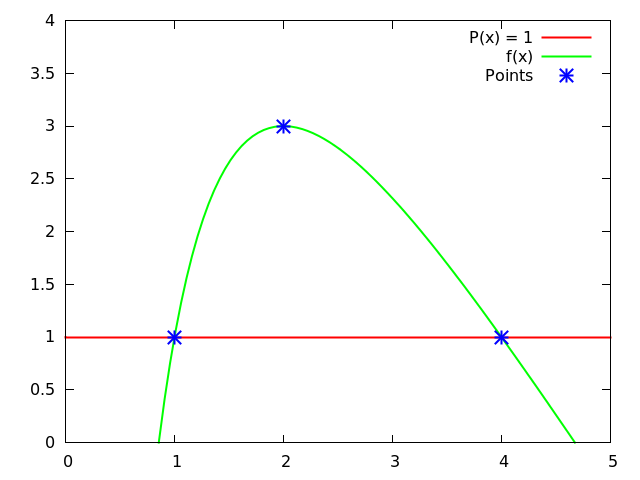
\includegraphics[height=.5\textheight]{p0.png}}
			\only<3>{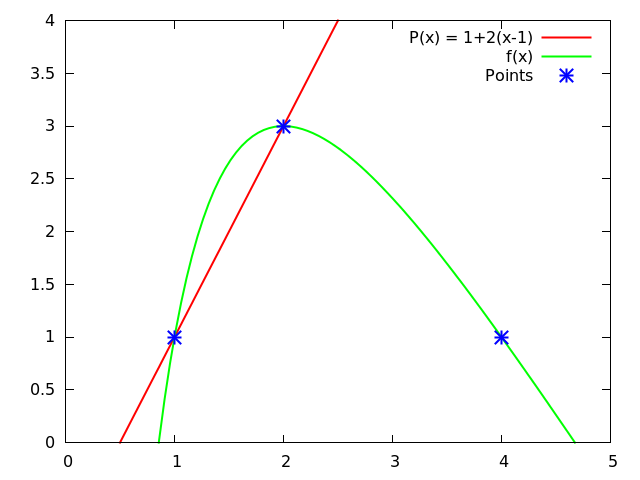
\includegraphics[height=.5\textheight]{p1.png}}
			\only<4>{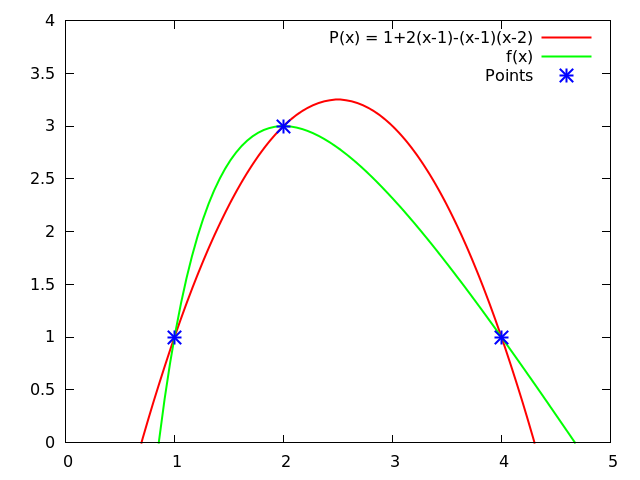
\includegraphics[height=.5\textheight]{p2.png}}
		\end{column}
	\end{columns}
\end{frame}

\begin{frame}
\frametitle{Разделенные разности}
	Ньютон нашел выражения для неизвестных коэффициентов $A$ в форме, удобной
	для практических вычислений. Для этого вводится понятие \emph{разделенной разности}.
	Разделенная разность $k$-го порядка обозначается как
	$f(\underbrace{x_p,x_q,\dots,x_s}_{k+1 \text{ аргумент}})$.
	Разделенные разности нулевого порядка совпадают со значениями самой функции в этой точке
	\[
	f(x_k) = f_k
	\]
	Остальные разности определяются рекуррентно:
	\[
	f(x_p,x_q,\dots,x_r,x_s) = \frac{f(x_q,\dots,x_r,x_s)-f(x_p,x_q,\dots,x_r)}{x_s - x_p}
	\]
	В этих обозначениях,
	\[
	P(x) = f(x_1) + f(x_1, x_2) (x-x_1) + f(x_1,x_2,x_3)(x-x_1)(x-x_2) + \dots
	\]
\end{frame}

\begin{frame}
\frametitle{Пример вычисления разделенных разностей}
	Вычисление разделенных разностей удобно проводить в виде таблицы:
	\pause
	\begin{table}
	\begin{tabular}{|c||c|c|c|c|c|c|}
	\hline
	$x_k$&
		\multicolumn{2}{p{1cm}}{\centering $\color<3,5>{blue!81!black}1$}&
		\multicolumn{2}{|p{1cm}}{\centering $\color<3,4>{blue!81!black}2$}&
		\multicolumn{2}{|p{1cm}|}{\centering $\color<4,5>{blue!81!black}4$}\\ \hline
	$f(x_k)$&
		\multicolumn{2}{p{1cm}}{\centering $\color<6>{blue}\color<3>{green!81!black}1$}&
		\multicolumn{2}{|p{1cm}}{\centering $\color<3,4>{green!81!black}3$}&
		\multicolumn{2}{|p{1cm}|}{\centering $\color<4>{green!81!black}1$}\\ \hline
	$f(x_k,x_{k+1})$&
		\multicolumn{1}{>{\columncolor[gray]{.5}}p{0.285cm}}{}&
		\multicolumn{2}{|p{1cm}}{\centering $\color<1,2>{white}\color<5,6>{green!81!black}
			\color<3>{red!81!black}2$}&
		\multicolumn{2}{|p{1cm}}{\centering $\color<1-3>{white}\color<5>{green!81!black}
			\color<4>{red!81!black}-1$}&
		\multicolumn{1}{|>{\columncolor[gray]{.5}}p{0.285cm}|}{}\\ \hline
	$f(x_k,x_{k+1},x_{k+2})$&
		\multicolumn{2}{>{\columncolor[gray]{.5}}p{1cm}}{}&
		\multicolumn{2}{|p{1cm}}{\centering $\color<1-4>{white}\color<5,6>{red!81!black}-1$}&
		\multicolumn{2}{|>{\columncolor[gray]{.5}}p{1cm}|}{}\\ \hline
	\end{tabular}
	\end{table}
	\only<1-2>{\[
	f(x_p,x_q,\dots,x_r,x_s) = \frac{f(x_q,\dots,x_r,x_s)-f(x_p,x_q,\dots,x_r)}{x_s - x_p}
	\]}
	\only<3>{\[
	{\color{red!81!black}f(x_1,x_2)} = \frac
		{{\color{green!81!black}f(x_2)}-{\color{green!81!black}f(x_1)}}
		{{\color{blue}x_2} - {\color{blue!81!black}x_1}}
	\]}
	\only<4>{\[
	{\color{red!81!black}f(x_2,x_3)} = \frac
		{{\color{green!81!black}f(x_3)}-{\color{green!81!black}f(x_2)}}
		{{\color{blue!81!black}x_3} - {\color{blue!81!black}x_2}}
	\]}
	\only<5>{\[
	{\color{red!81!black}f(x_1,x_2,x_3)} = \frac
		{{\color{green!81!black}f(x_2,x_3)}-{\color{green!81!black}f(x_1,x_2)}}
		{{\color{blue!81!black}x_3} - {\color{blue!81!black}x_1}}
	\]}
	\only<6>{\[
	\phantom{\frac{\phantom{f(x)}}{\phantom{f(x)}}}
	P(x) = {\color{blue!81!black} 1} + {\color{green!81!black} 2}(x-x_1)
		{\color{red!81!black}-1}(x-x_1)(x-x_2)
	\phantom{\frac{\phantom{f(x)}}{\phantom{f(x)}}}
	\]}
\end{frame}

\subsection{Форма Лагранжа}
\begin{frame}
\frametitle{Базисные интерполяционные полиномы}
	Решим вспомогательную
	\begin{block}{Задачу о базисном интерполяционном многочлене}
		Необходимо построить многочлен, который во всех точках $x_k$, кроме точки $x_j$ обращался в 0,
		а в точке $x_j$ был равен $1$
		\[
		\ell_j(x_k) = \delta_{kj} =
		\begin{cases}
		0,& k\neq j\\
		1,& k = j
		\end{cases}
		\]
	\end{block}
	\pause
	Поскольку степень этого многочлена $n-1$, а $x_k, k\neq j$ --- его корни,
	то сам многочлен можно записать в форме
	$$
	\ell_j(x) = A(x-x_1)(x-x_2)\cdots(x-x_{j-1})(x-x_{j+1})\cdots(x-x_n)
	$$
	\pause
	Пользуясь условием $\ell_j(x_j) = 1$
	$$
	\ell_j(x) = \frac{(x-x_1)(x-x_2)\cdots(x-x_{j-1})(x-x_{j+1})\cdots(x-x_n)}
		{(x_j-x_1)(x_j-x_2)\cdots(x_j-x_{j-1})(x_j-x_{j+1})\cdots(x_j-x_n)}
	$$
\end{frame}

\begin{frame}
\frametitle{Интерполяционный многочлен в форме Лагранжа}
	Используя базисные интерполяционные многочлены Лагранжа легко написать
	явное выражение для интерполянта в форме Лагранжа
	\[
	P(x) = \sum_{j=1}^n \ell_j(x) f_j
	\]
	\pause
	Действительно,
	\[
	P(x_k) = \sum_{j=1}^n \ell_j(x_k) f_j = \ell_k(x_k) f_k = f_k
	\]
	\pause
	Заметим, что базисные интерполяционные многочлены $\ell_j(x)$ зависят только
	от \emph{сетки}, а не от значений функции в узлах. Если приходится решать
	несколько задач интерполяции на одной и той же сетке, то форма Лагранжа может
	оказаться удобнее.
\end{frame}

\begin{frame}
\frametitle{Пример вычисления базисных многочленов}
	\[
	\begin{array}{|c||c|c|c|}
	\hline
	x_k&1&2&4\\	\hline
	f_k&1&3&1\\	\hline
	\end{array}
	\]
	\begin{columns}[T]
		\begin{column}{0.55\textwidth}
		\vspace{-0.5cm}
		\begin{align*}
		\ell_1(x) = \frac{(x-2)(x-4)}{(1-2)(1-4)} = \frac{1}{3}(x-2)(x-4)\\
		\ell_2(x) = \frac{(x-1)(x-4)}{(2-1)(2-4)} = \frac{1}{2}(x-1)(4-x)\\
		\ell_3(x) = \frac{(x-1)(x-2)}{(4-1)(4-2)} = \frac{1}{6}(x-1)(x-2)
		\end{align*}
		\end{column}
		\begin{column}{0.45\textwidth}
		\centering
		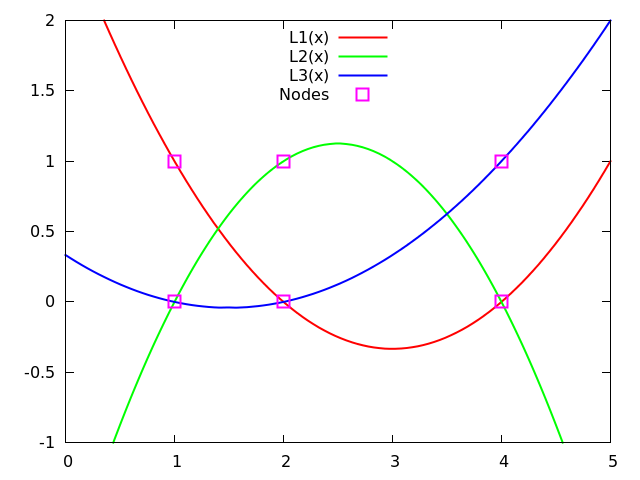
\includegraphics[height=.37\textheight]{l.png}
		\end{column}
	\end{columns}
	\pause

	\begin{block}{Вопрос}
		Чему равна сумма $\ell_1(x) + \ell_2(x) + \ell_3(x)$ ?
		\pause

		$\ell_1(x) + \ell_2(x) + \ell_3(x) \equiv 1$.

		Подсказка: рассмотреть $f(x) \equiv 1$ и ее интерполянт $P(x)$
	\end{block}
\end{frame}

\begin{frame}
\frametitle{Пример интерполяционного многочлена}
	\begin{center}
	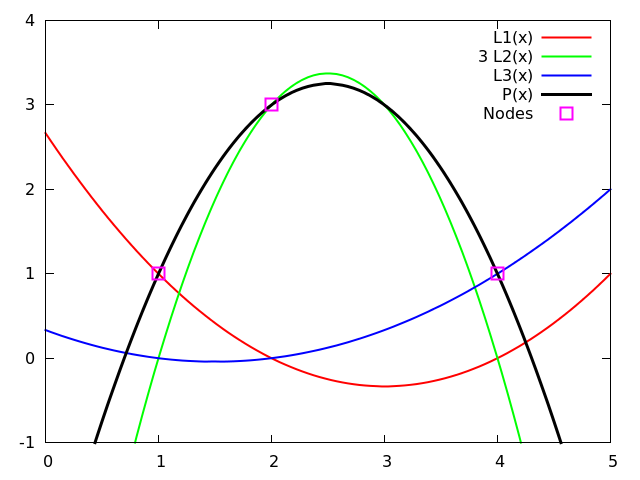
\includegraphics[height=0.65\textheight]{lp.png}
	\end{center}
	\[
		P(x) = \frac{1}{3}(x-2)(x-4) + 3\frac{1}{2}(x-1)(4-x) + \frac{1}{6}(x-1)(x-2)
	\]
\end{frame}

\subsection{Погрешность интерполяции}
\begin{frame}
\frametitle{Погрешность алгебраической интерполяции}
	Логичный вопрос --- насколько восстановленная по значениям функция (интерполянт)
	близка к исходной? Она в точности с ней совпадает в точках $x_k$, но что можно сказать
	про различия в промежутках?
	\pause

	\begin{block}{Теорема}
	Ошибка алгебраической интерполяции допускает оценку
	$$
	\left| f(x) - P(x) \right| \leqslant \frac{|f^{(n)}(\xi)|}{n!}|\omega(x)| \leqslant \frac{M_n}{n!} |\omega(x)|, \quad x,\xi,x_k \in [a,b],
	$$
	где $\omega(x) = (x-x_1)(x-x_2)\cdots(x-x_n)$
	\end{block}
	\pause
	Часть ошибки $\frac{M_n}{n!}$ зависит только от вида функции, а вторая $\omega(x)$ ---
	только от расположения узлов интерполяции.
\end{frame}

\begin{frame}
\frametitle{Ошибка интерполяции на равномерной сетке}
	Рассмотри равномерную сетку $x_k = a + \frac{k-1}{n-1} (b-a)$
	Оценим максимальное значение функции $|\omega(x)|$ на ней.
	\[
	\max_{x \in [a,b]} |\omega(x)| \leqslant (n-1)!
		\left(\frac{b-a}{n-1}\right)^n \equiv (n-1)! h^n,
	\]
	где через $h$ обозначен шаг сетки, то есть $\frac{b-a}{n-1}$
	\pause

	Отсюда, погрешность интерполяции, которая является ошибкой метода, равна
	\[
	\varepsilon_{\text{метод}} = \frac{M_n}{n!} \max_{x \in [a,b]}| \omega(x) |
		\leqslant \frac{M_n}{n} h^n
	\]
	Однако, в ошибке метода фигурирует максимум $n$-й производной, который
	может сильно расти при увеличении $n$.
\end{frame}

\begin{frame}
\frametitle{Интерполяция функции Рунге на равномерной сетке}
	\begin{figure}[ht!]
	\centering
	\only<1>{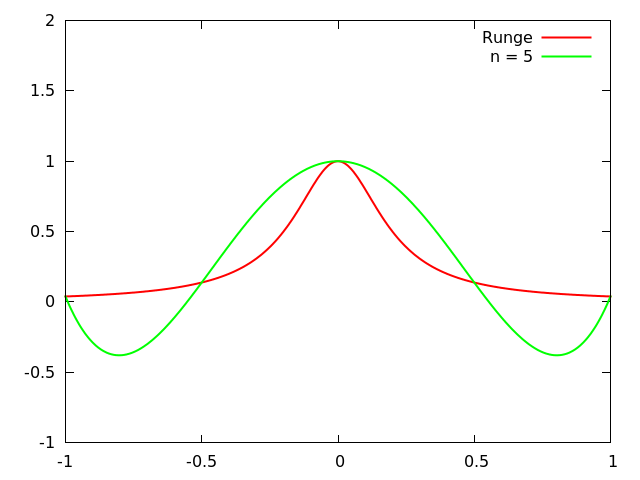
\includegraphics[height=0.7\textheight]{runge5.png}}%
	\only<2>{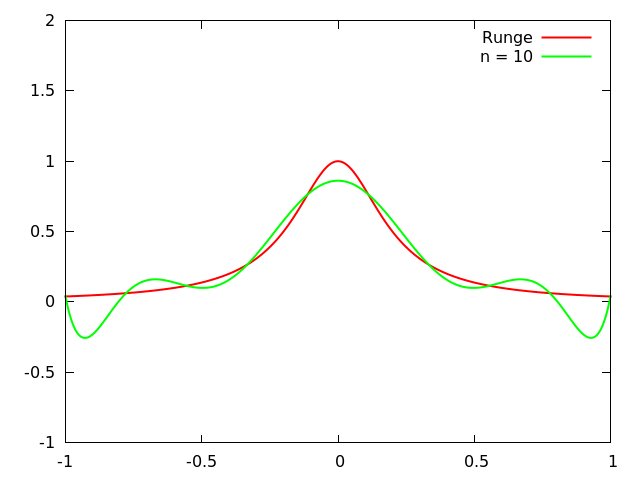
\includegraphics[height=0.7\textheight]{runge10.png}}%
	\only<3>{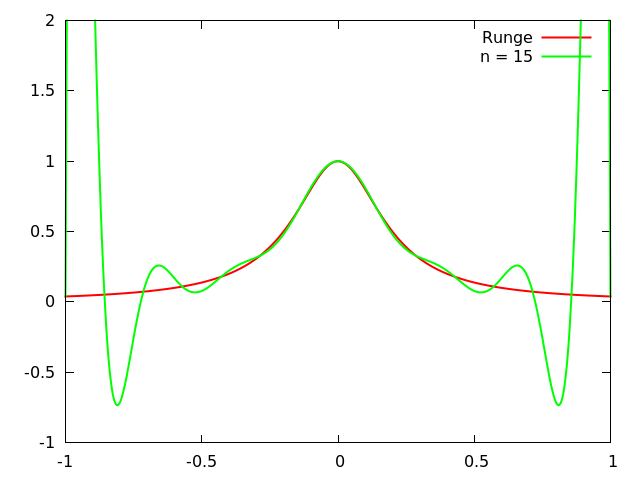
\includegraphics[height=0.7\textheight]{runge15.png}}%
	\only<4>{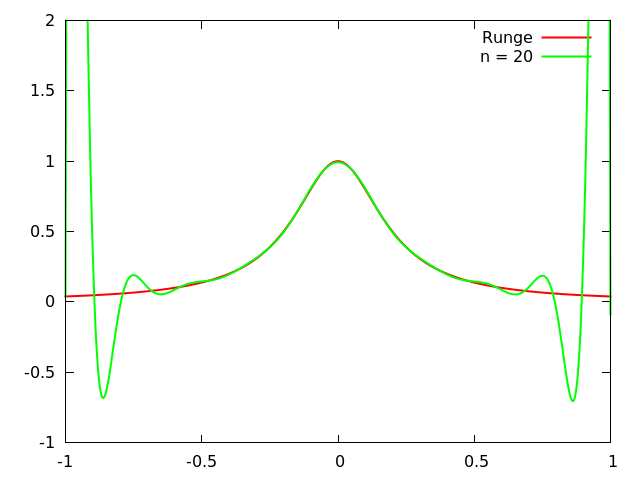
\includegraphics[height=0.7\textheight]{runge20.png}}%
	\only<5>{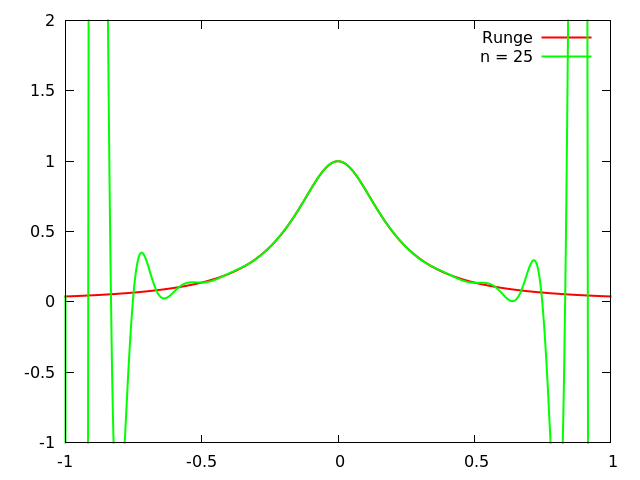
\includegraphics[height=0.7\textheight]{runge25.png}}%
	\end{figure}
	\[f(x) = \dfrac{1}{1 + 25x^2}\]
\end{frame}

\subsection{Расположение узлов интерполяции}
\begin{frame}
\frametitle{Оптимальный выбор узлов интерполяции}
	Посмотрим, насколько возможно уменьшить ошибку интерполяции, только за счет
	выбора узлов $x_k$. (Предполагаем, что можем узнать	только $n$ значений функции,
	но в тех точках, которые нам интересны).
	\pause

	Задача состоит в минимизации функции $\omega(x)$ за счет выбора $x_k$.

	Если искать минимум максимума модуля $\omega(x)$, то такая задача была решена Чебышевым(1881)%
	\footnote{\textit{Чебышев П.Л.} О функциях мало удаляющихся от нуля при некоторых величинах
		переменной - Спб.,1881}

	\[
	\max_{x \in [a,b]} \left| (x-x_1)(x-x_2) \cdots (x-x_n) \right| \rightarrow \min_{x_k}
	\]
\end{frame}

\begin{frame}
\frametitle{Многочлены Чебышева}
	Многочленом Чебышева степени $n$ называется многочлен
	\[
	T_n(x) = \cos n \arccos x = 2^{n-1} x^n + \dots
	\]
	Он является многочленом, наименее уклоняющимся от нуля на отрезке $[-1,1]$ среди
	многочленов с тем же коэффициентом при старшей степени.
	Чтобы получить решение предыдущей задачи, необходимо этот многочлен отмасштабировать
	и перевести отрезок $[-1,1]$ в $[a,b]$.
	\pause

	\[
	\omega(x) = \widetilde{T}_n(x) = \frac{(b-a)^n}{2^{2n-1}} \cos n \arccos \frac{2x-a-b}{b-a}
	\]

	\pause
	$$
	\max_{x\in[a,b]} |\omega(x)| = \frac{(b-a)^n}{2^{2n-1}} =
	\frac{h^n n^n}{2^{2n-1}} \approx \frac{h^n n! e^n}{2^{2n-1}\sqrt{2\pi n}} =
	h^n n! \left(\frac{e}{4}\right)^n \sqrt\frac{2}{\pi n}
	$$

	Существенное отличие от равномерной сетки в быстро убывающем при $n
	\rightarrow \infty$ сомножителе $\left(\frac{e}{4}\right)^n$
\end{frame}

\begin{frame}
\frametitle{Сетка из нулей многочлена Чебышева}
	Узлы сетки $x_k$ являются корнями $\omega(x)$. Оптимальной в смысле минимума ошибки интерполяции будет
	сетка из узлов $x_k$, которые являются корнями $\omega(x) = \tilde{T}_n(x)$.
	\pause
	\begin{columns}[T]
	\begin{column}{0.6\textwidth}
	\begin{gather*}
	\tilde{T}_n(x) = \frac{(b-a)^n}{2^{2n-1}}
		\cos n \arccos \frac{2x-a-b}{b-a}\\
	x_k = \frac{a+b}{2} + \frac{b-a}{2} \cos \left(\frac{2k-1}{2n}\pi\right)
	\end{gather*}
	\end{column}
	\begin{column}{0.4\textwidth}
	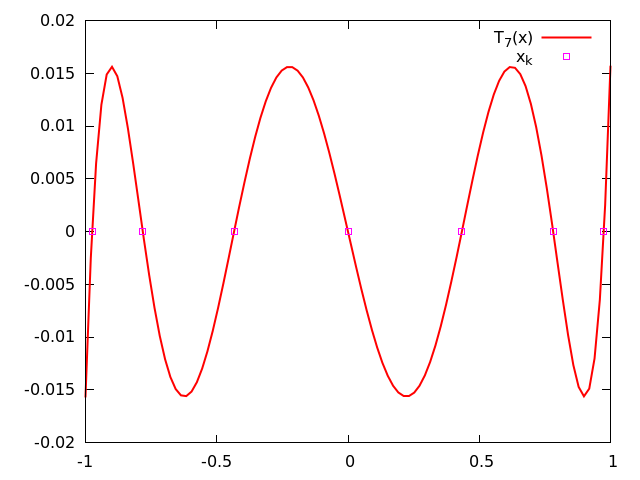
\includegraphics[height=0.3\textheight]{cheb.png}
	\end{column}
	\end{columns}
	\pause

	\begin{block}{Теорема}
		Если функция $f(x)$ имеет ограниченную производную на отрезке, то последовательность
		интерполяционных многочленов $P_n(x)$ на такой сетке сходится равномерно к $f(x)$.
		\[
		P_n(x) \rightrightarrows f(x)
		\]
	\end{block}
\end{frame}

\begin{frame}
\frametitle{Интерполяция функции Рунге на чебышевской сетке}
	\begin{figure}[ht!]
	\centering
	\only<1>{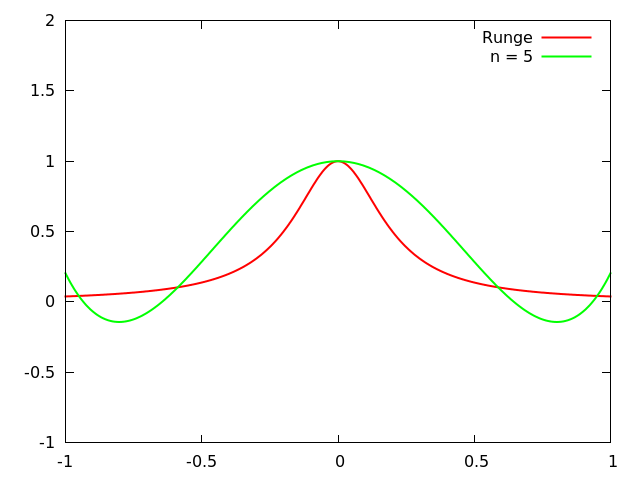
\includegraphics[height=0.7\textheight]{runge5_ch.png}}%
	\only<2>{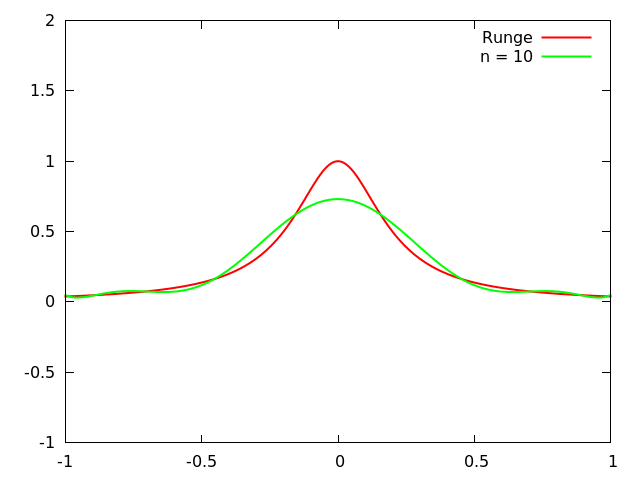
\includegraphics[height=0.7\textheight]{runge10_ch.png}}%
	\only<3>{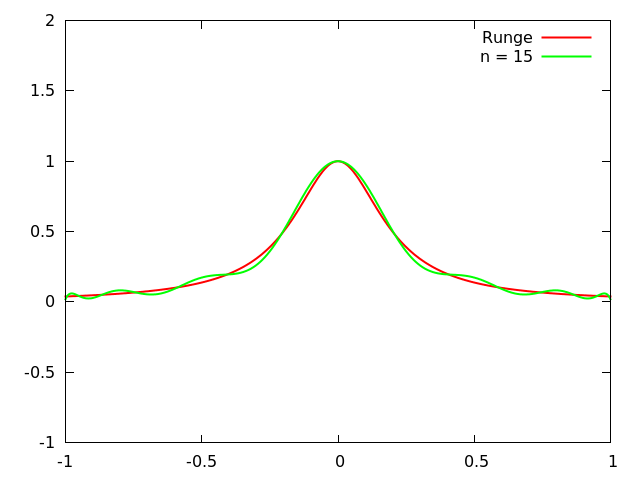
\includegraphics[height=0.7\textheight]{runge15_ch.png}}%
	\only<4>{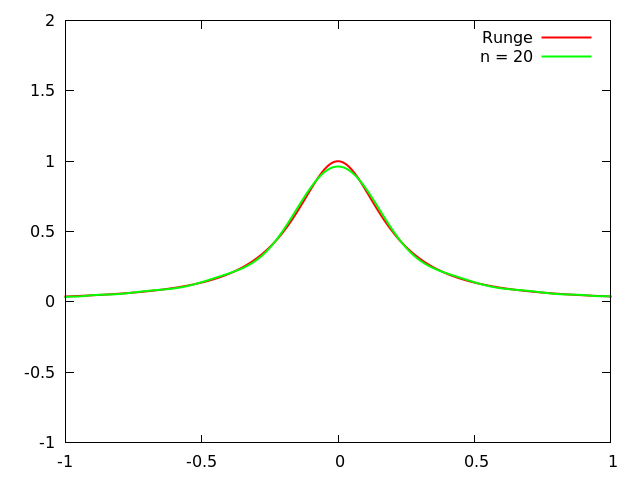
\includegraphics[height=0.7\textheight]{runge20_ch.png}}%
	\only<5>{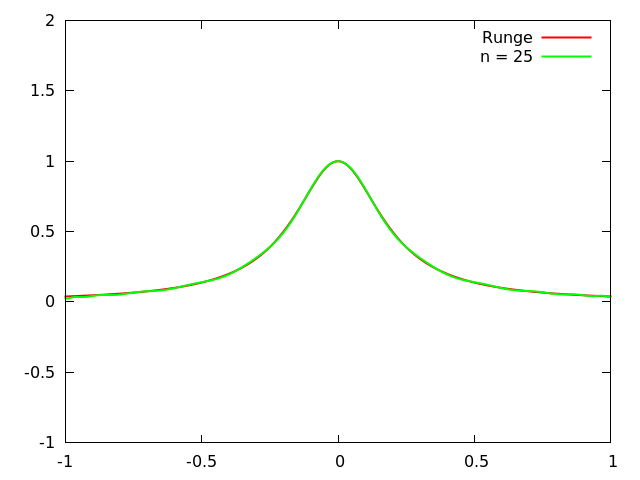
\includegraphics[height=0.7\textheight]{runge25_ch.png}}%
	\end{figure}
	\[f(x) = \dfrac{1}{1 + 25x^2}\]
\end{frame}


\subsection{Экстраполяция}
\begin{frame}
\frametitle{Экстраполяция}
	До сих пор, мы изучали поведение интерполянта в пределах отрезка, на котором заданы точки.
	Также можно ставить задачу определения значений функции за пределами отрезка, например,
	спрогнозировать значения функции по уже имеющимся данным.
	\pause

	Большая часть формальных выводов, в том числе и погрешности экстраполяции,
	один-к-одному переносятся из интерполяции. Отличие заключается в расширении отрезка $[a,b]$,
	до отрезка, в который входит точка $x$. В свою очередь, оценки для максимумов функции $\omega(x)$
	сильно зависят от изучаемого отрезка.
\end{frame}

\begin{frame}
\frametitle{Экстраполяция на равномерной сетке}
	Для оценки ошибки экстраполяции остается верной формула
	\[
	\varepsilon_{\text{метод}} \leqslant \frac{M_n}{n!} |\omega(x)|
	\]
	Пусть точка $x$ лежит правее точки $b$ на $\delta$: $x = b + \delta$
	\[
	\omega(x) = \prod_{k=0}^{n-1} \left(\delta+kh\right) =
		h^n\frac{\Gamma\left(\frac{\delta}{h}+n\right)}{\Gamma\left(\frac{\delta}{h}\right)}
	\approx
	\begin{cases}
		h^n n!,& \delta \lesssim h\\
		\delta^n,& \delta \gg h
	\end{cases}
	\]
	То есть, экстраполяция на расстояния порядка $h$ имеет погрешность, близкую к погрешности интерполяции,
	но по мере удаления от конца отрезка, ошибка стремительно растет.
\end{frame}

\begin{frame}
\frametitle{Экстаполяция на сетке из нулей многочлена Чебышева}
	В этом случае открывается другое экстремальное свойство многочленов Чебышева.
	\pause

	Наряду с тем, что на данной сетке функция $\omega(x)$ наименее отклоняется от нуля
	среди всех многочленов с коэффициентом $1$ при старшей степени, эта функция
	стремительнее всех остальных растет за пределами отрезка $[a,b]$.
	\pause

	Таким образом, сетка из нулей многочлена Чебышева оказывается самой плохой
	в смысле погрешности экстраполяции --- оценка для ошибки превышает оценку
	для ошибки на любой другой сетке.
\end{frame}

\subsection{Чувствительность интерполяции}
\begin{frame}
\frametitle{Чувствительность интерполяции}
	Возьмем $20$ точек функции $\sin x$ и чуть-чуть (на доли процента)
	пошевелим значение функции в одной из них
	\begin{columns}
	\begin{column}[c]{0.75\textwidth}

	% comments MATTER!!!!! Keep 'em ----------------------------VVV
	\only<1>{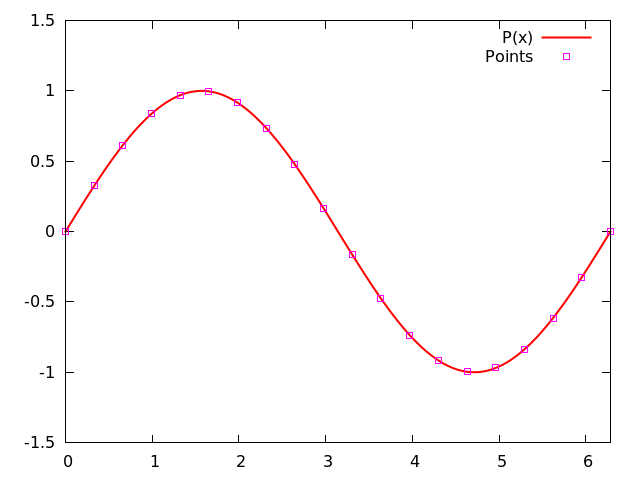
\includegraphics[width=1.00\textwidth]{sense0.png}}%
	\only<2>{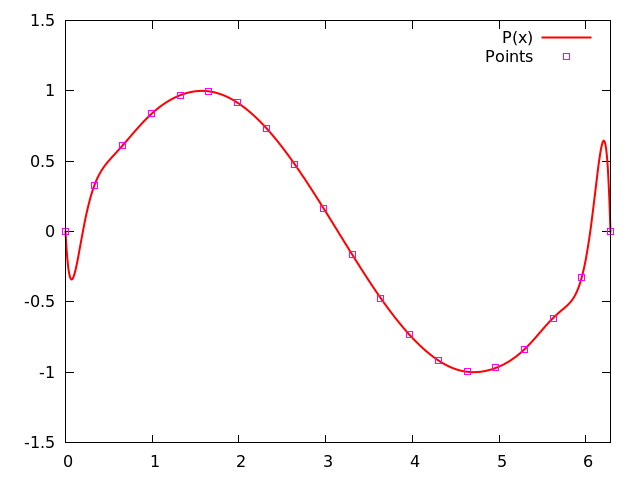
\includegraphics[width=1.00\textwidth]{sense2.png}}%
	\only<3>{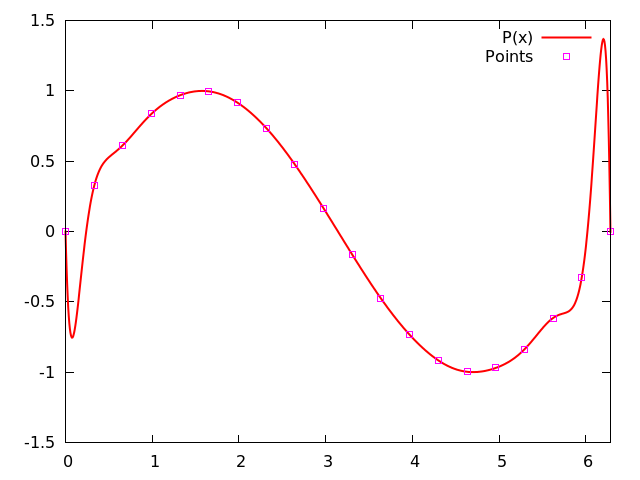
\includegraphics[width=1.00\textwidth]{sense4.png}}%
	\only<4>{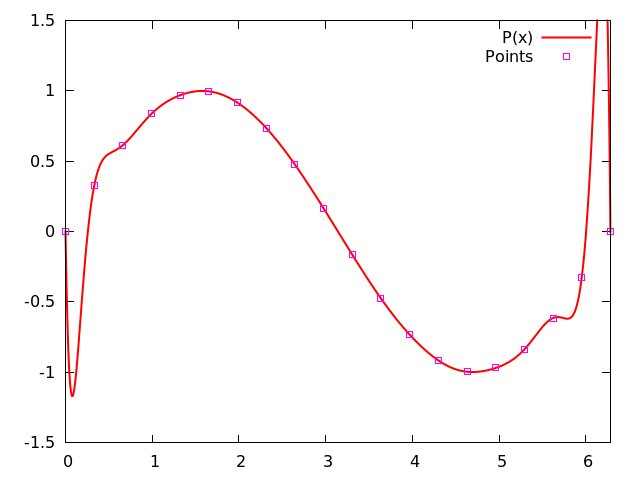
\includegraphics[width=1.00\textwidth]{sense6.png}}%
	\only<5>{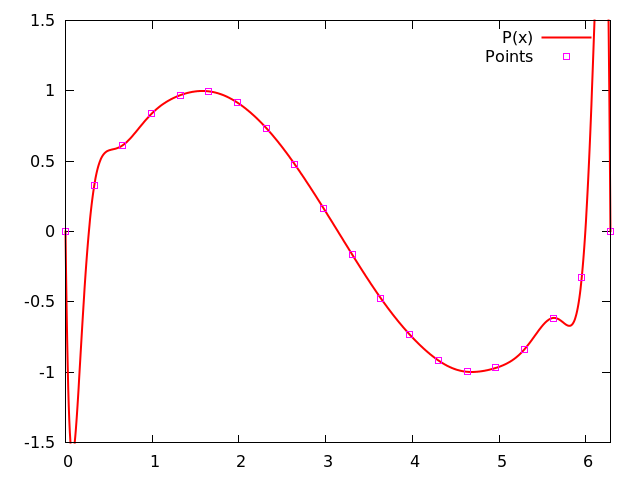
\includegraphics[width=1.00\textwidth]{sense8.png}}%
	\only<6>{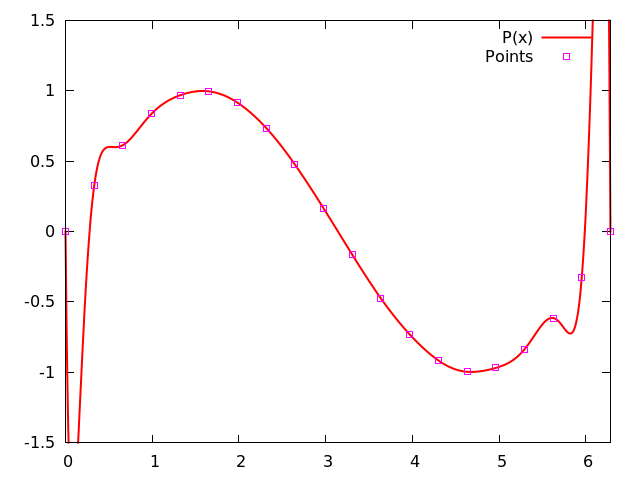
\includegraphics[width=1.00\textwidth]{sense10.png}}%
	\only<7>{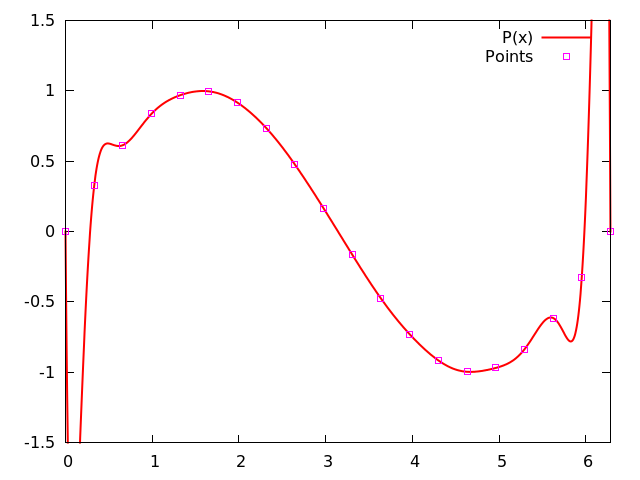
\includegraphics[width=1.00\textwidth]{sense12.png}}%
	\only<8>{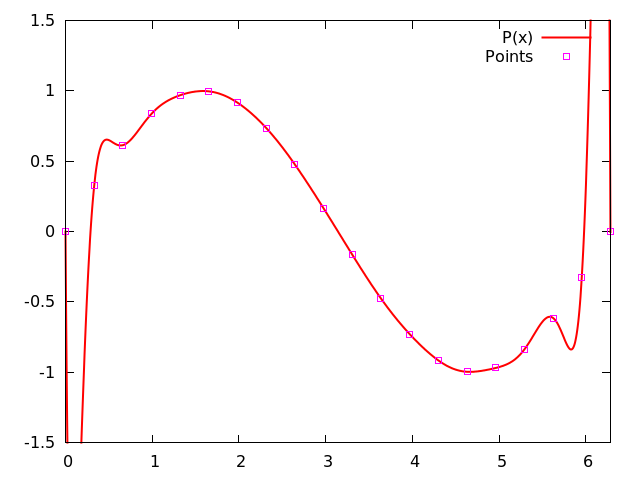
\includegraphics[width=1.00\textwidth]{sense14.png}}%
	\only<9>{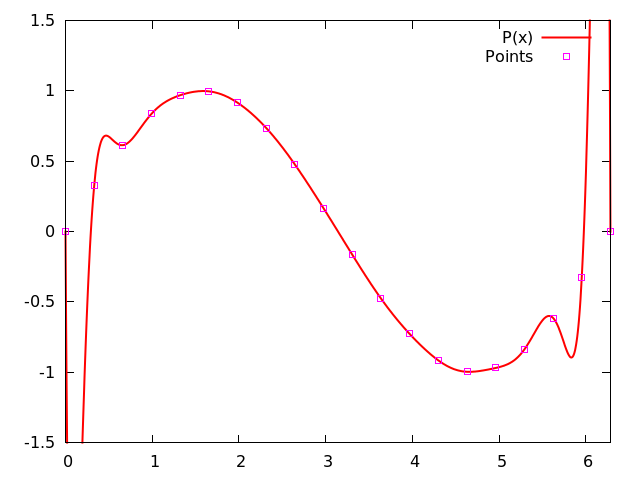
\includegraphics[width=1.00\textwidth]{sense16.png}}%
	\only<10>{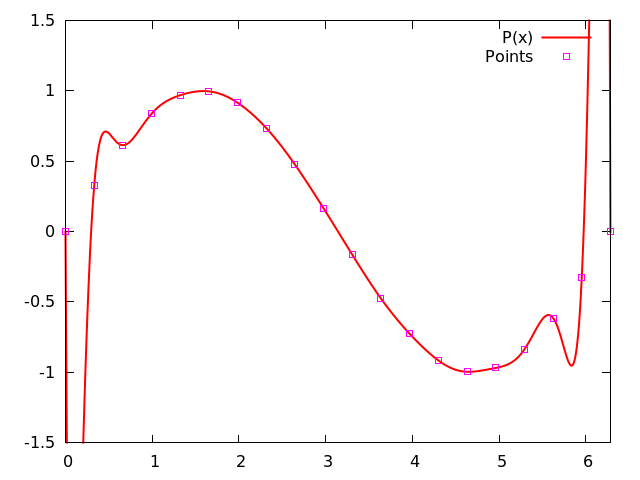
\includegraphics[width=1.00\textwidth]{sense18.png}}%
%	\only<11>{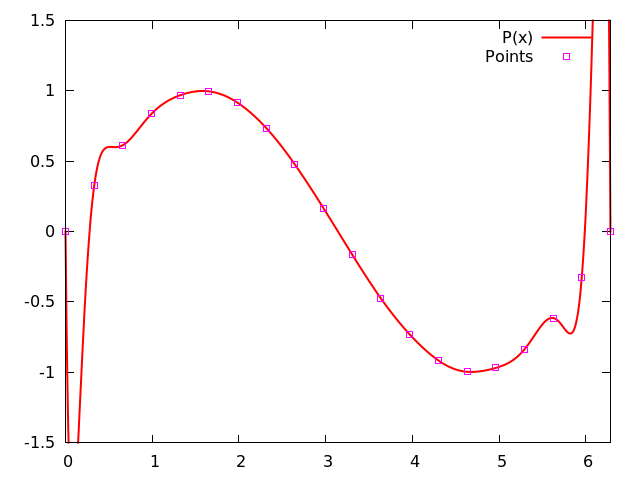
\includegraphics[width=1.00\textwidth]{sense10.png}}%
%	\only<12>{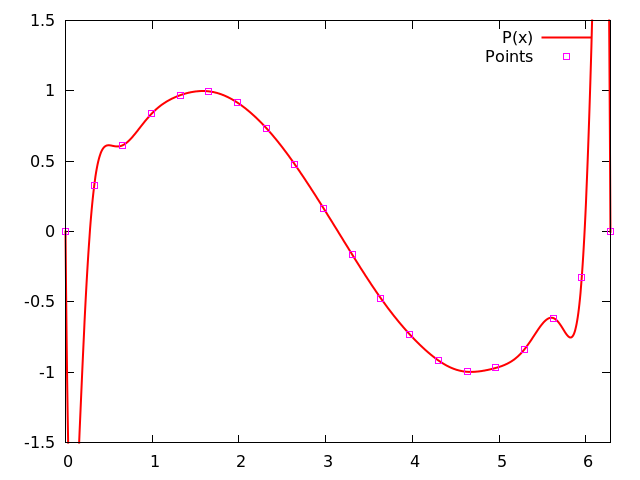
\includegraphics[width=1.00\textwidth]{sense11.png}}%
%	\only<13>{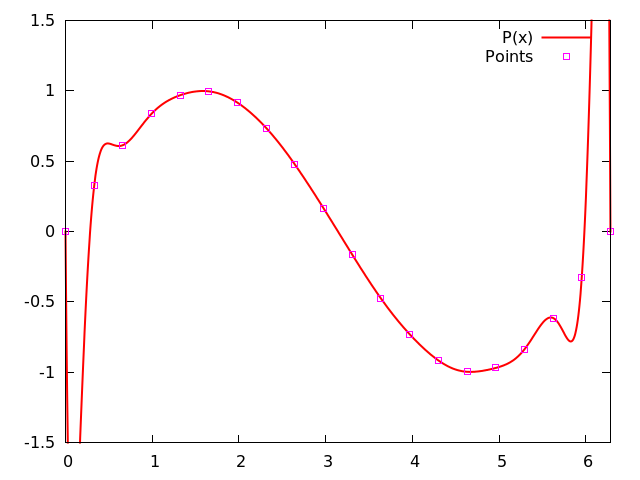
\includegraphics[width=1.00\textwidth]{sense12.png}}%
%	\only<14>{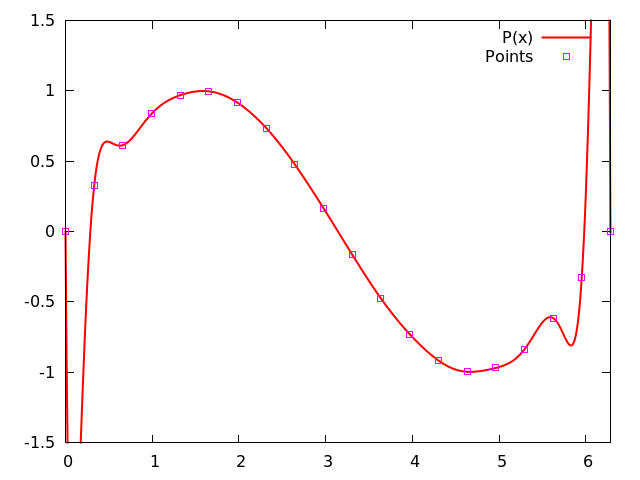
\includegraphics[width=1.00\textwidth]{sense13.png}}%
%	\only<15>{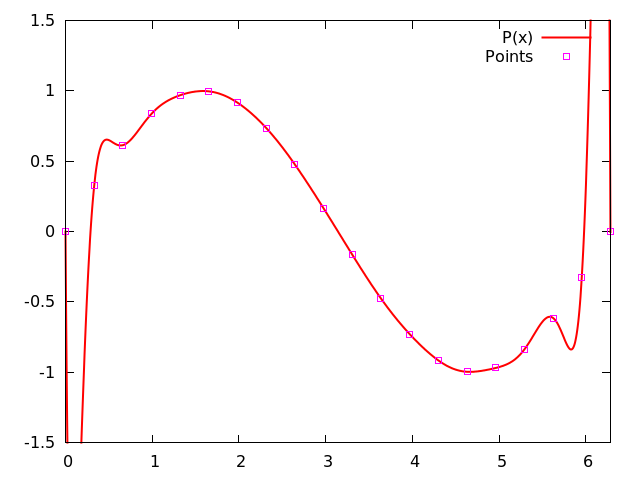
\includegraphics[width=1.00\textwidth]{sense14.png}}%
%	\only<16>{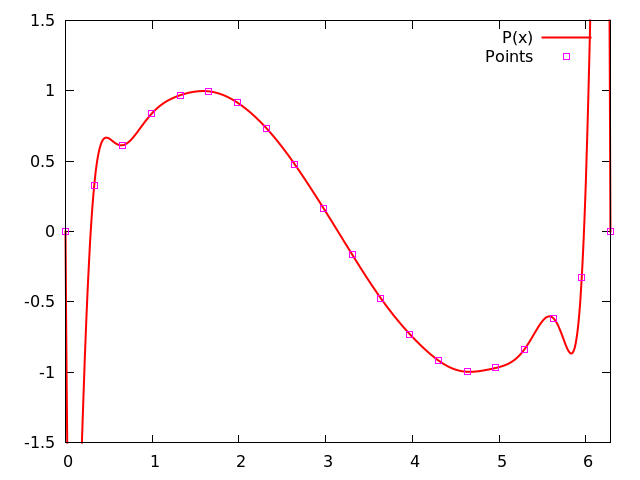
\includegraphics[width=1.00\textwidth]{sense15.png}}%
%	\only<17>{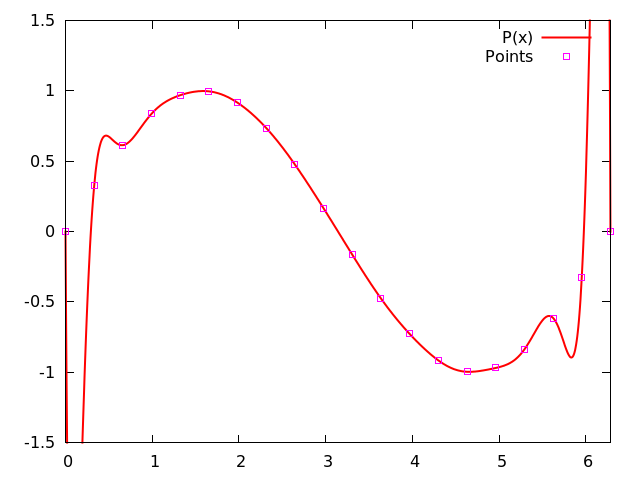
\includegraphics[width=1.00\textwidth]{sense16.png}}%
%	\only<18>{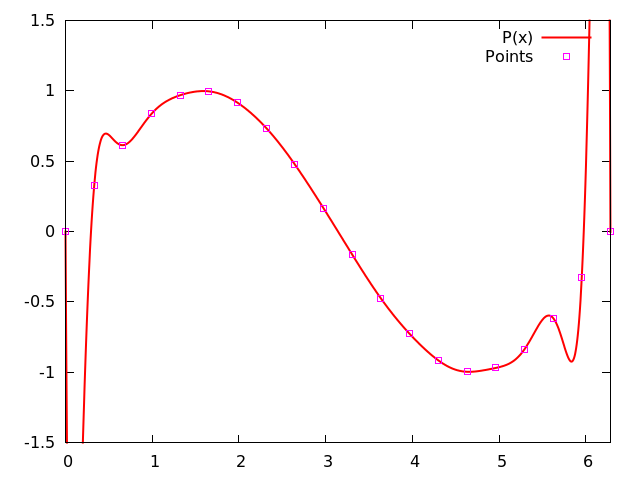
\includegraphics[width=1.00\textwidth]{sense17.png}}%
%	\only<19>{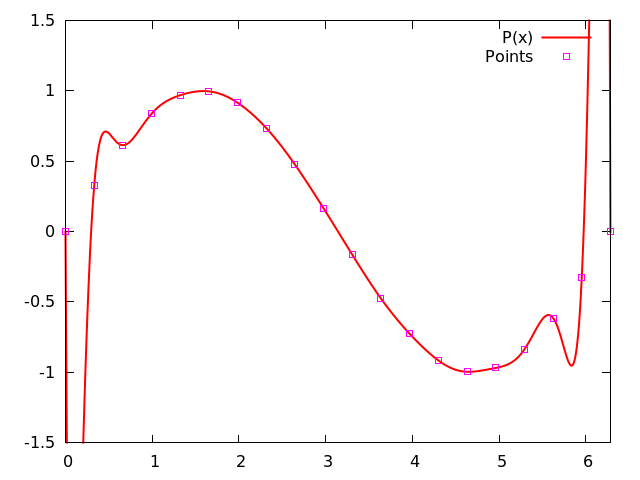
\includegraphics[width=1.00\textwidth]{sense18.png}}%
%	\only<20>{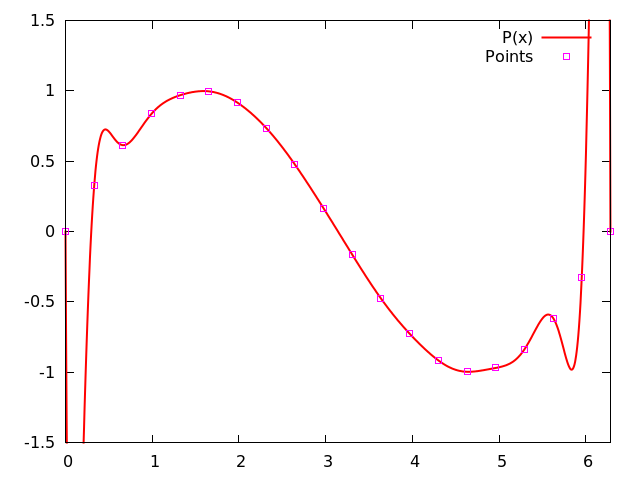
\includegraphics[width=1.00\textwidth]{sense19.png}}%

	\end{column}
	\begin{column}[c]{0.25\textwidth}

	\invisible<1>{\hyperlink{jumptofirst}{\beamergotobutton{К первому кадру}}}

	\invisible<10>{\hyperlink{jumptolast}{\beamergotobutton{К последнему кадру}}}

	\end{column}
	\end{columns}

	\hypertarget<1>{jumptofirst}{}
	\hypertarget<10>{jumptolast}{}
\end{frame}

\begin{frame}
\frametitle{Чувствительность интерполяции}
	Вспомним выражение для интерполяционного многочлена в форме Лагранжа
	\[
	P(x) = \sum_{j=1}^n f_j \ell_j(x)
	\]
	<<Пошевелив>> $f_k$ на $\delta f_k$, мы тем самым <<пошевелили>> интерполянт на
	\[
	\delta P(x) = \sum_{j=1}^n (f_j+\delta f_j) \ell_j(x) - \sum_{j=1}^n f_j \ell_j(x) = \sum_{j=1}^n \delta f_j \ell_j(x)
	\]
	Поскольку конкретное направление шевеления (в большую или меньшую сторону) обычно неизвестно, а известно только
	абсолютное значение, можно написать оценку
	\[
	|\delta P(x)| \leqslant \sum_{j=1}^n |\delta f_j| |\ell_j(x)|
	\]
\end{frame}

\begin{frame}
\frametitle{Функция Лебега и константа Лебега}
	Рассмотрим случай, когда все $|\delta f_k|$ одинаковы и равны $\delta f$:
	\[
	|\delta P(x)| \leqslant \delta f \sum_{j=1}^n |\ell_j(x)|
	\]
	Сумма $\sum_{j=1}^n |\ell_j(x)|$ зависит только от сетки, называется \emph{функцией Лебега} этой сетки и обозначается $L(x)$.
	В случае, когда интересует максимальное отклонение интерполянта по всему отрезку, вводят максимум функции Лебега,
	который называется \emph{константой Лебега} и обозначается $L$
	\[
	|\delta P(x)| \leqslant L(x) \delta f
	\]
	\[
	|\delta P| \leqslant \max_{x \in [a,b]} L(x)  \delta f \equiv L \delta f
	\]
\end{frame}

\begin{frame}
\frametitle{Функция Лебега равномерной сетки}
	\begin{figure}%
	\only<1>{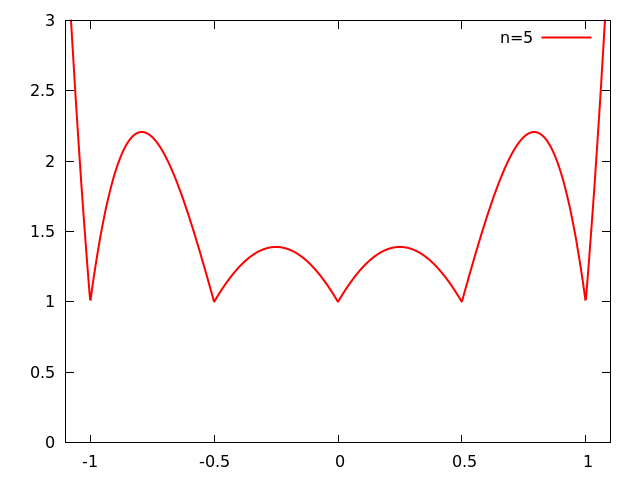
\includegraphics[height=0.45\textheight]{leb_un5.png}}%
	\only<2>{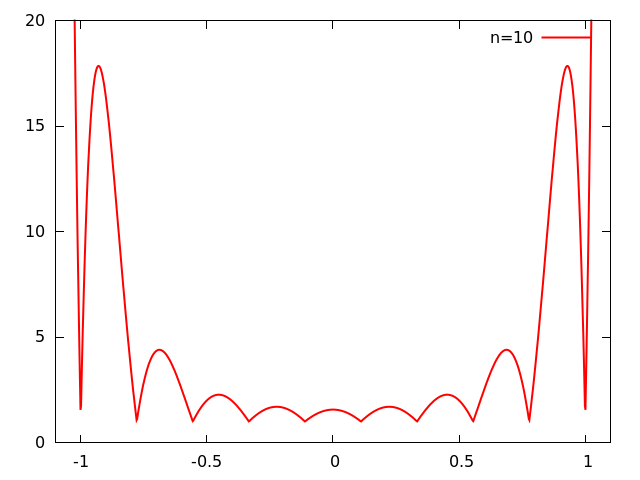
\includegraphics[height=0.45\textheight]{leb_un10.png}}%
	\only<3->{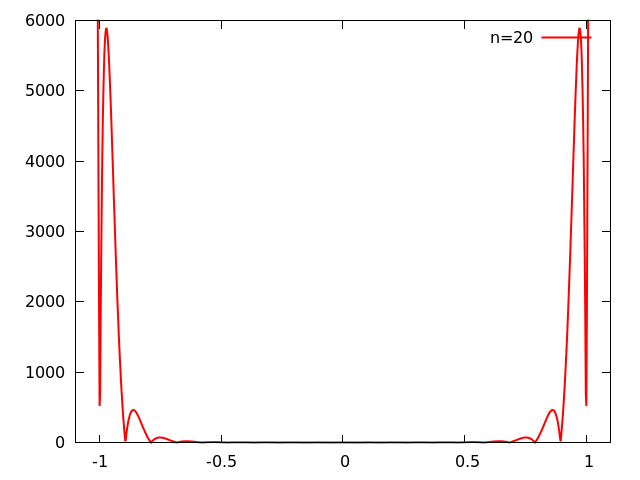
\includegraphics[height=0.45\textheight]{leb_un20.png}}%
	\caption{
	\only<1>{При $n = 5$ константа Лебега $L \approx 2.25$}%
	\only<2>{При $n = 10$ константа Лебега $L \approx 18$}%
	\only<3->{При $n = 20$ константа Лебега $L \approx 6000$}%
	}
	\end{figure}

	Для равномерной сетки константа Лебега $L$ растет как $L \sim \frac{2^n}{\sqrt{n}}$.

	\uncover<4>{
	Также видно, что за пределами отрезка функция Лебега растет еще быстрее.
	Это означает что задача экстраполяции крайне чувствительна
	к заданию точных значений в узлах.
	}
\end{frame}

\begin{frame}
\frametitle{Функция Лебега сетки из нулей многочлена Чебышева}
	\begin{figure}%
	\only<1>{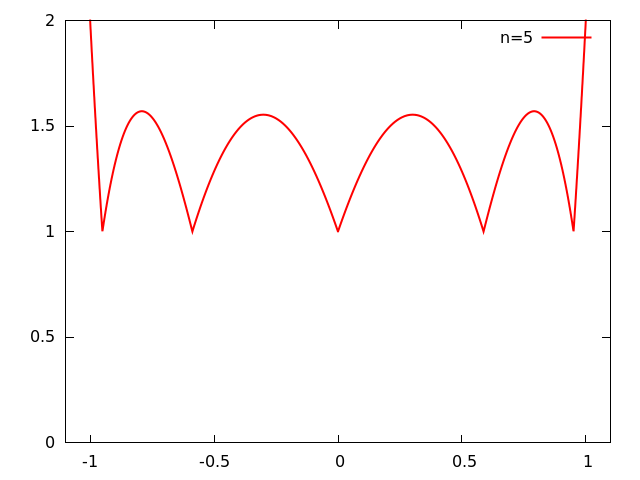
\includegraphics[height=0.5\textheight]{leb_ch5.png}}%
	\only<2>{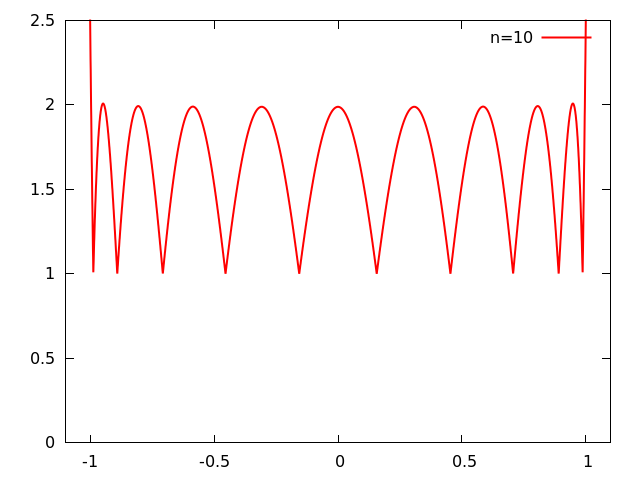
\includegraphics[height=0.5\textheight]{leb_ch10.png}}%
	\only<3->{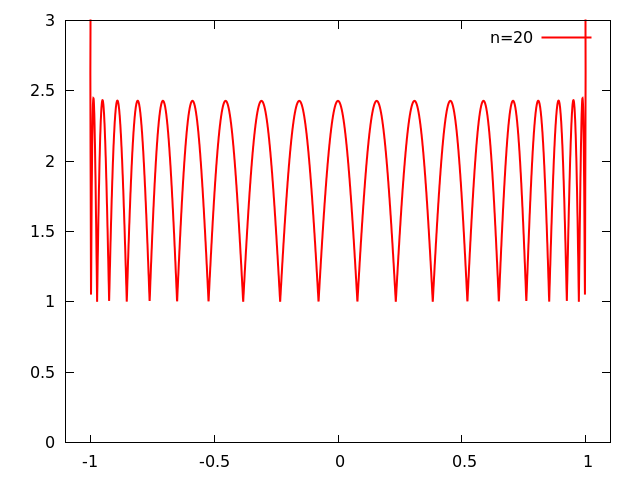
\includegraphics[height=0.5\textheight]{leb_ch20.png}}%
	\caption{
	\only<1>{При $n = 5$ константа Лебега $L \approx 1.6$}%
	\only<2>{При $n = 10$ константа Лебега $L \approx 2$}%
	\only<3->{При $n = 20$ константа Лебега $L \approx 2.5$}%
	}
	\end{figure}

	Для этой сетки константа Лебега $L$ растет как $L \sim \frac{2}{\pi}\ln n$.
	\pause

	Использование сетки из нулей многочлена Чебышева позволяет сильно снизить требования к
	точности задания функции в узлах.
\end{frame}

\section{Сплайны}
\begin{frame}
\frametitle{Проблемы глобальной интероляции}
	Глобальная алгебраическая интерполяция при большом количестве
	узлов начинают испытывать проблемы при быстром росте констант $M_n$ и весьма
	чувствительна к заданию функции в узлах.

	\pause
	Одно из решений --- проводить не глобальную, а локальную интерполяцию,
	по небольшому количеству соседних узлов. Такой интерполянт называется сплайном.

	\pause
	\begin{itemize}
	\item \emph{Степенью сплайна} называется степень многочлена на каждом отрезке.
	\item \emph{Гладкостью сплайна} называется количество непрерывных производных у функции на \emph{всем} отрезке
	\item \emph{Дефектом сплайна} называется разность между степенью и гладкостью сплайна.
	\end{itemize}
\end{frame}

\begin{frame}
\frametitle{Кусочно-линейная интерполяция}
	Простейшая кусочно-многочленная интерполяция --- кусочно линейная.
	Функция на каждом отрезке приближается линейной.

	\begin{columns}[c]
	\begin{column}{0.6\textwidth}
	\begin{figure}
	\center
	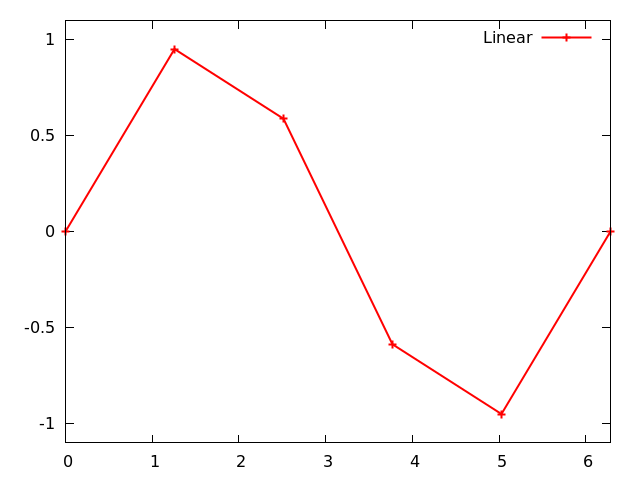
\includegraphics[width=\textwidth]{spline1_1.png}%
	\end{figure}
	\end{column}
	\begin{column}{0.4\textwidth}
	Степень --- 1

	Гладкость --- 0

	Дефект --- 1
	\end{column}
	\end{columns}
\end{frame}

\begin{frame}
\frametitle{Кусочно-квадратичная интерполяция}
	Построим на каждом отрезке параболу по трем ближайшим точкам.
	\begin{columns}[c]
	\begin{column}{0.6\textwidth}
	\begin{figure}
	\center
	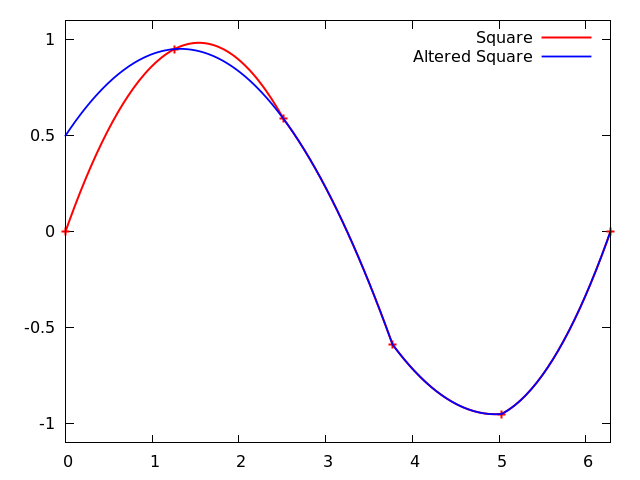
\includegraphics[width=\textwidth]{spline2_2.png}%
	\end{figure}
	\end{column}
	\begin{column}{0.4\textwidth}
	Степень --- 2

	Гладкость --- 0

	Дефект --- 2
	\end{column}
	\end{columns}
\end{frame}

\begin{frame}
\frametitle{Гладкая кусочно-квадратичная интерполяция}
	Построим по трем первым точкам параболу, а на следующих отрезках будем стоить параболу, проходящую
	через концы отрезка и гладко продолжающую параболу на предыдущем отрезке.

	Пусть $P_k(x) = a_kx^2+b_kx+c$, $q_k = P'_{k-1}(x_k)$
	\[
	\left\{
	\begin{array}{lcl}
		a_kx_k^2+b_kx_k+c_k &=& f_k\\
		a_kx_{k+1}^2+b_kx_{k+1}+c_k &=& f_{k+1}\\
		2a_kx_k+b_k &=& q_k\\
	\end{array}
	\right.
	\]
	%$$
	%\left\{
	%\begin{array}{lcl}
		%a_k &=&  \frac{f_{k+1}-f_k+q(x_{k}-x_{k+1})}{(x_{k+1}-x_k)^2}\\
		%b_k &=&  \frac{2x_k(f_{k}-f_{k+1})+q(x_{k+1}^2-x_k^2)}{(x_{k+1}-x_k)^2}\\
		%c_k &=&  \frac{f_{k+1}x_{k}^2+x_{k+1}\left(qx_k(x_k-x_{k+1})+f_k(x_{k+1}-2x_k)\right)}{(x_{k+1}-x_k)^2}\\
		%q_{k+1} &=&  \frac{f_{k+1}-f_k}{x_{k+1}-x_k} - q_k
	%\end{array}
	%\right.
	%$$
	Данный метод позволяет строить сплайны любой степени с дефектом 1. Частный случай степени 3 называется сплайном Шонберга.
\end{frame}

\begin{frame}
\frametitle{Гладкая кусочно-квадратичная интерполяция}
	\begin{columns}[c]
	\begin{column}{0.6\textwidth}
	\begin{figure}
	\center
	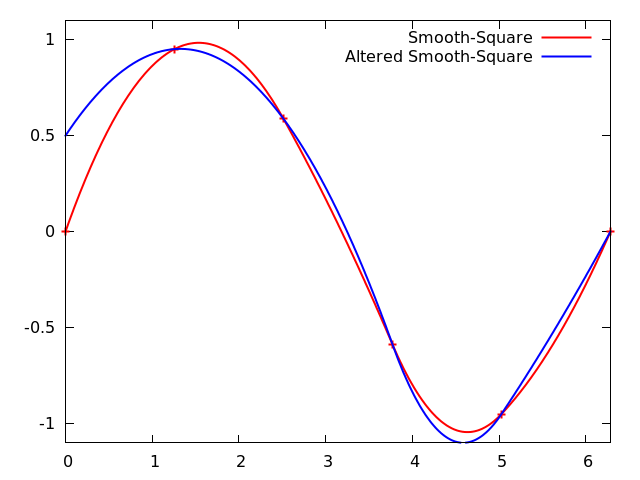
\includegraphics[width=\textwidth]{spline2_1.png}%
	\end{figure}
	\end{column}
	\begin{column}{0.4\textwidth}
	Степень --- 2

	Гладкость --- 1

	Дефект --- 1
	\end{column}
	\end{columns}

	Удалось добиться гладкости сплайна, но при этом исчезло свойство локальности:
	при изменении какого-нибудь значения функции изменяется весь сплайн. Конечно, изменение не такое
	большое, как при глобальной интерполяции, но хотелось бы от него избавиться
\end{frame}

\begin{frame}
\frametitle{Локальные гладкие сплайны}
	Возьмем за основу негладкий сплайн $P(x)$(например кусочно-линейный).
	На каждом отрезке будем искать кубическую параболу $Q_k(x)$, которая проходит через его концы,
	на левом конце производная совпадает с $P'(x_k+0)$, а на правом --- с $P'(x_{k+1}+0)$.
	Таким образом, производная сплайна будет непрерывной, а для вычисления интерполянта на
	отрезке используются только 3 ближайшие точки
	$$
	\left\{
	\begin{array}{lcl}
		Q_k'(x_k) &=& \frac{f_{k}-f_{k-1}}{x_k-x_{k-1}}\\
		Q_k'(x_{k+1}) &=& \frac{f_{k+1}-f_{k}}{x_{k+1}-x_{k}}\\
		Q_k(x_k) &=& f_k\\
		Q_k(x_{k+1}) &=& f_{k+1}\\
	\end{array}
	\right.
	$$
	Таким образом можно строить локальные сплайны степени $2s+1$ при гладкости $s$.
\end{frame}

\begin{frame}
\frametitle{Гладкая локальная кусочно-кубическая интерполяция}
	\begin{columns}[c]
	\begin{column}{0.6\textwidth}
	\begin{figure}
	\center
	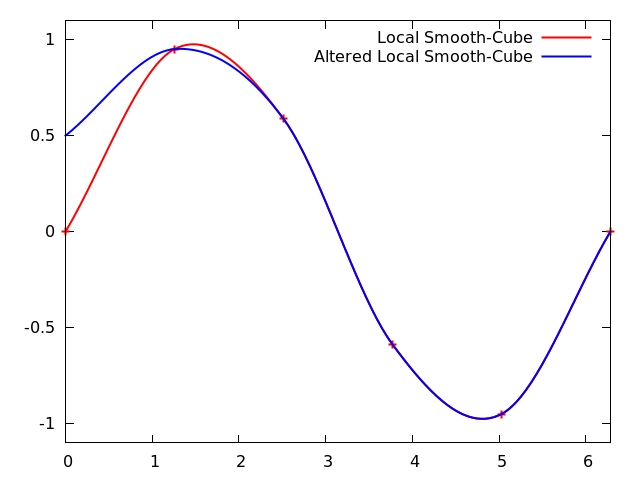
\includegraphics[width=\textwidth]{spline3_1.png}%
	\end{figure}
	\end{column}
	\begin{column}{0.4\textwidth}
	Степень --- 3

	Гладкость --- 1

	Дефект --- 2
	\end{column}
	\end{columns}

	Сплайн получился гладкий и сохранил свойство локальности. Такие локальные сплайны называются сплайнами В.С. Рябенького.
\end{frame}

\begin{frame}[plain]
  \begin{center}
  {\Huge Спасибо за внимание!}
  \vspace{8ex}

  Цыбулин Иван

  e-mail: \colorhref{mailto:tsybulin@crec.mipt.ru}{tsybulin@crec.mipt.ru}
  \end{center}
\end{frame}

\end{document}
